%%% Local Variables:
%%% mode: latex
%%% TeX-master: t
%%% End:

\documentclass[doctor]{thuthesis}
% \documentclass[%
%   bachelor|master|doctor, % mandatory option
%   xetex|pdftex|dvips|dvipdfm, % optional
%   secret,
%   openany|openright,
%   arialtoc,arialtitle]{thuthesis}

% 所有其它可能用到的包都统一放到这里了,可以根据自己的实际添加或者删除。
\usepackage{thutils}

\hypersetup{bookmarksopenlevel=0}

% 你可以在这里修改配置文件中的定义,导言区可以使用中文。
% \def\myname{薛瑞尼}

\begin{document}

% 定义所有的eps文件在 figures 子目录下
\graphicspath{{figure/}}


%%% 封面部分
\frontmatter
% vim:textwidth=70

%%% Local Variables:
%%% mode: latex
%%% TeX-master: t
%%% End:
\secretlevel{绝密} \secretyear{2100}

\ctitle{分布式系统管理与调试关键问题的研究}
% 根据自己的情况选,不用这样复杂
\makeatletter
\ifthu@bachelor\relax\else
  \ifthu@doctor
    \cdegree{工学博士}
  \else
    \ifthu@master
      \cdegree{工学硕士}
    \fi
  \fi
\fi
\makeatother


\cdepartment[计算机]{计算机科学与技术系}
\cmajor{计算机科学与技术}
\cauthor{高崇南} 
\csupervisor{郑纬民教授}
% 如果没有副指导老师或者联合指导老师,把下面两行相应的删除即可。
% 日期自动生成,如果你要自己写就改这个cdate
%\cdate{\CJKdigits{\the\year}年\CJKnumber{\the\month}月}
\cdate{\CJKdigits{2009}年\CJKnumber{4}月}

\etitle{Research on Key Problems on Distributed System Management and Debugging}

% \edegree{Doctor of Science} 
\edegree{Doctor of Engineering} 
\emajor{Computer Science and Technology} 
\eauthor{Chongnan Gao} 
\esupervisor{Professor Weimin Zheng} 
% 这个日期也会自动生成,你要改么?
\edate{April, 2009}

% 定义中英文摘要和关键字
\begin{cabstract}

% 800-1000汉字

  分布式系统成为了支撑Internet服务的关键组成部分,随着系统规模越来越大,
  系统处理逻辑日趋复杂,有效的管理与调试分布式系统成为了挑战。目前相关
  研究取得了一些进展,但很多关键问题尚待解决。本文针对分布式系统自管理
  机制、自动推断分布式系统层次结构任务模型的方法等方面进行了研究,取得
  了有价值的研究成果。

  本文主要贡献包括:

  \begin{enumerate}

    \item 使分布式应用管理系统可自管理的机制。分布式系统需要被管理。分
    布式应用管理系统帮助人们简化了部署与维护分布式系统的负担。为了有效
    的完成管理任务,管理系统本身也是一个分布式应用,需要被管理,已有的
    工作还没有很好的解决这个问题。本文提出了使管理系统具备自管理机制的
    方法,并实现了一个可自管理的分布式应用管理系统SMON。SMON能够自动将
    自己安全部署到一组指定的机器上去,将自己从运行错误中恢复,并在线升
    级自己至新版本。

    \item 自动推断系统层次结构任务模型的方法。分布式系统难于调试,理解
    系统的运行时行为是分析解决系统正确性与性能问题关键。已有的方法可以
    帮助人们理解系统运行时的因果路径,但是需要手工标注代码,使用困难且
    需要使用者对系统有深入了解。本文提出了一种完全不需要人工帮助,自动
    推断系统层次结构任务模型的方法。使用得到的层次结构任务模型,可以对
    系统设计有深入的了解,并帮助分析导致系统缺陷的原因。

    \item 利用系统日志,推断系统层次任务模型的方法。日志是由系统开发人
    员创建的,因此它们包含了关键的系统状态和事件信息。利用这些信息,可
    以帮助推断应用层语意的任务关系。本文的推断方法能够自动从无结构的系
    统日志中提取任务信息,并推断任务之间的层次结构关系。使用得到的任务
    层次关系,可以帮助理解系统设计,解决系统已有的性能问题。

  \end{enumerate}

\end{cabstract}

\ckeywords{分布式系统; 自管理; 层次结构任务模型; 日志分析}

\begin{eabstract}
  Distributed systems are the key components in today's Intertnet
  services. While the system scale goes larger and the processing
  logic becomes more complex, it is a challenge to managing and
  debugging large scale distributed systems. While current research
  work makes great progresses, some key problems are still not fully
  resolved yet. In this thesis, we conducted research on
  self-management of distributed systems and automatically inferrence
  of hierarchical task models of distributed systems.

  The contributions of this thesis are:

  \begin{enumerate}

    \item Mechanism of adding self-management property for distributed
    application management systems. Distributed systems need
    management. The distributed application management system
    simplifies tasks in deploying and maintaining distributed systems.
    To efficiently accomplish management tasks, management system is
    itself an distributed applicaiton, which needs to be managed too.
    Existing work doesn't address the problem very well. In this
    theis, a mechanism to support self-management of distributed
    application management system is proposed and a self-managed
    distributed application managment system (SMON) is designed. SMON
    can automatically and securely deploy itself to a set of machines,
    recover itself from failure automatically and upgrade itself to
    newer versions online.

    \item Methodology of automatic inferrence of hierarchical tasks
    models for distributed system. It is a challenge to debug
    distributed systems and understanding the runtime behaviour is the
    key to solve the correctness and performance bug. Existing tools
    require manual annotation, which is hard to use and poses a high
    bar on the user. In this thesis, an automatic inference
    methodology of hierarchical task models for distributed systems is
    developed. The hierarchical task models help on understanding of
    system design and implementation, and help on finding root cause
    of system correctness and performance bugs.

    \item Methodology of inferrence of hierarchical task models based
    on system log. Logs are created by system developers and contain
    key information on system states and events. Using the
    information, we can understand the relations among application
    level tasks. The inference methodology can extract task
    information from unstructured system logs automatically and
    inferrence hierarchical relations among the tasks. The
    hierarchical task models help on understanding of system design
    and implementation, and help on finding root cause of system
    correctness and performance bugs.

  \end{enumerate}

\end{eabstract}

\ekeywords{Distribute System; Self-Management; Hierarchical Task
Model; Log Analysis}

\makecover

% 目录
\tableofcontents

% 符号对照表
\begin{denotation}

\item[instrumentation] 插装
\item[bug] 软件错误、缺陷
\item[failure] 故障、失败、失效
\item[network partition] 网络分割
\item[primitive] 原语
\item[heuristic (n.)] 启发
\item[predicate] 谓词
\item[invariant] 不变量
\item[model-checking] 模型验证
\item[replay] 回放

\end{denotation}



%%% 正文部分
\mainmatter
% vim:tw=60

\section{Introduction}
\label{sec:intro}

As industry is moving towards \textit{cloud computing}, many
players in the industry are building large and complex data
center applications on top of clusters of commodity PCs.
Ensuring the correctness and performance of the applications
are critical to providing sustained service to clients.
However, bugs have been challenging service developers and
maintainers continually.

However, the inherent complexity of the system hinders
people from understanding the system easily. The system are
usually built in a tiered fashion, with each tier providing
certain abstraction to the upper layer. Within a logical
tier, its function is implemented as a distributed system.
It may consist of hundreds or thousands of distributed
processes which works coorperately to fulfill the requests
from upper tier. Within a particular process, asynchronous
staged handling of messages is well adopted to fully utilize
the computing resource on a node. By leveraing the above
techniques, developers have built large scale of complex
systems to serve requests worldwide. The handling of a
request is splitted into pieces of tasks which are executed
distrbutedly across tiers, processes and stages. 

Understanding runtime behaviour of the complex system is key
to verify system design, debug its correctness and
performance problems. By tracking task pieces and their
causal dependencies, we can construct task flow by linking
together pieces of its execution throughout the system.  In
our previous work, we further developed techniques to
automatically tracking tasks and infer hierarchical task
models. Using the task models, developers can better
understand the structures of components and their
dependencies, and use debugging tools to instrument the
system and verify the behavior of tasks at appropriate
layers.

The production system contains abundant logging information
on system status, but it is not fully explored yet. It is
useful for two reason. First, the log is added by developers
who are familiar with the system.  The resulting log is a
faithful records of system runtime behaviour. Second, log
usually contains both state report and high level
descriptions. The derived task models is of value for both
automatic processing and human understanding.

The hierarchical structure of tasks is often consist with
the hierarchy of data processed by tasks. For example. In
cosmos, data are organized as streams and streams are
consisted of extents. By inspecting cosmos logs, task that
processing a stream is splitted into subtasks. The first
subtask do some stream level processing (open, etc.), and
the following tasks process extents in the stream. But the
task boundaries are not marked in the log.

By mining and leveraging data hierarchy, we can use the
information to infer the task hierarchy. A log item which
starts to process a stream marks the begin of a task. The
task lasts before the log item which process another stream.
Within the task, it is splitted into subtasks at
extent-processing boundary.

In this paper, we present a method for automatically infer
data hierarchy recorded in system log and use the
information to construct task models.  We also describe our
experiences in using the inferred task models to
understanding the system design and debug performance
problems.

\comment{
It faces several challenges. First, logs are not
written in well strucutured form. Second, log contains a lot
information other than data identifer, and the noises must
be reduce automatically with best effort.

}

\comment{
and build hierarchical task models to better
understand and check system runtime behaviour.

Meanwhile, debugging correctness and performance problems
for the systems are difficult.

System log is a rich source of information for understanding
system runtime behaviour.

Researchers have proposed several techniques, but system log
is not explored much.

In this paper, we try to build hierarchical task model
through logs.

Contribution/Highlights:

Goal: Understanding system behaviour by exploiting existing
system logs

magpie: more details on low level properties d3s: customized
log point pip: manual annotation

our advangtage: 

existing log more on high level semantic
}

\section{Design}
\label{sec:design}

In this section, we describe the detailed process of mining
data hierarchy using system log. It works in two phases.

\subsection{Extract key-value pairs}
\notes{value format are limited, we can find value part
easily, and track back in the text to find its key name.}

\subsection{Mining hierarchical relation of keys}

\notes{
\begin{itemize}
\item rule 1: keyS $>$ keyP, then keyS comes before keyP
\item rule 2: keyS $>$ keyP, then there're 1-to-many mapping relation between keyS and keyP value set.
\end{itemize}
}

\subsection{Construct hierarchical task models}
\notes{In this step, we summarize the key relations into
partial orders. and use it to construct task models.}

\section{Discussion}
\label{sec:discussion}
Discussion. \notes{topic need decided}

\section{Experiences}
\label{sec:exp}

\subsection{Understanding system behaviour}
\notes{understanding cosmos client, en and csm, but the
dependency line may be missing. Because log doesn't contain
enough information to join tasks among threads.}

\subsection{Guide on debugging}
\notes{
using the model to guide on debugging cosmos network
library.

}

\section{Related Works}
\label{sec:related}
Related Works

\section{Conclusion}
\label{sec:conclusion}
Conclusion

\section{References}
\label{sec:ref}
References


% vim:tw=60

\section{Related Works}
\label{sec:related}
Related Works \cite{Lamport1978}



% vim:textwidth=70
\chapter{可自管理的分布式应用管理系统}
\label{chap:selfman}

%问题,相关工作,创新点,基本\textbf{方法},实验

%问题提出:管理系统是一个分布式应用,同样需要管理
%
%目前的办法:集中部署启动管理系统到各个机器上,并集中式探测、维护(需要
%确认,或者说确定目前方法的缺陷)
%
%集中式的:plush,smartfrog,app-manager,globus,cfengine,还有
%
%plush, app-manager, smartfrog, cfengine, globus, amazon ec2
%
%==========
%为什么要管理管理系统:部署是必须的。更新是必须的。监测呢?可以用cron。
%
%ec2上可以用预装了plush的AMI
%
%攻击点:部署和更新也不经常有,监测死活可以用cron,管理节点死了几个也没事,
%早晚会发现,在那么大规模上,节点多几个少几个没太大问题。
%
%目前管理管理系统的办法有什么不足:
%
%一个可能得点:象self-host文章说的那样,说app希望可以改变运行的节点
%===========
%
%基本方法:节点相互探测对方状态,依据探测的结果,进行相应的管理步骤,实现
%
%系统的自管理。
%
%挑战:可扩展,鲁棒稳定,支持安全的自动认证,扩展管理能力(?)
%
%设计理念:简单、无状态(microreboot?)

\section{本章引言}

分布式系统~\cite{Ghemawat2003,DeCandia2007}是当今internet服务~
\cite{google, amazon?}的关键组成部分。随着普通计算机硬件成本越来越低,
搭建一个规模成百上千的分布式计算平台是很普通的事情。一些常见的分布式计
算平台包括Planet-Lab~\cite{Bavier2004}, Amazon
EC2~\cite{Garfinkel2007} and Teragrid~\cite{Catlett2002}。这些计算平台
可以提供大容量的存贮能力和巨大的计算能力,因此,设计良好的应用可以充
分利用这些资源来提升自己的性能。

随着分布式应用的规模越来越大,有效的管理它们越来越有挑战性。分布式应用
管理系统就是用来简化部署和维护分布式应用的系统。为了有效的完成管理
任务,管理系统也被设计为一个复杂的分布式系统。一个管理系统包括运行在不
同机器上的若干“节点\footnote{对于采用集中式算法的管理系统,节点就是所
谓的客户端}”。这些管理节点间形成一个覆盖网络,节点相互合作来部署分布
式应用。当分布式应用被部署并启动以后,这些管理节点可以监测并维护运行在
同一机器内的应用节点。管理员可以通过管理系统查询应用的状态,或者按照需
求向应用发送控制命令。

我们注意到,由于管理系统实际上也是一个分布式系统,或者说分布式应用,这
带来了一个重要的问题:管理系统也需要被管理。首先,需要把管理节点部署到
一组机器上去,其次,\note{这里需要想想怎么说}

在本文中,我们提出了可自管理的覆盖网络(SMON, Self-Managed Overlay
Network)。SMON是一个新颖的分布式应用管理系统,它具有内建自管理能力,
包括自我部署、自我更新和自我恢复能力。因而,它有效的解决了分布式管理系
统也需要管理的问题。SMON包括分布在一组机器上的管理节点,这些节点相互探
测对方的状态,依据探测的结果,自动执行自我管理任务,包括安装新的SMON管
理节点、更新SMON管理节点至新的版本,或者恢复失败的SMON管理节点。这样,
从整体来看,SMON具有了自我管理的能力。

作为一个分布式应用管理系统,SMON提供了一组基本的管理语意。\note{应用管
理,拓展管理能力。}

设计SMON需要解决一下几个挑战性问题。

首先,SMON需要有良好的可扩展性。其次,为了让SMON节点能够自动在远程机器
上安装新的SMON节点,或者恢复失败的节点,需要有安全机制使SMON节点能够自
动与远程机器认证并登陆,同时保护用户的认证信息(例如私钥)不会被泄露。
最后,SMON的管理能力应该是能够被拓展的。

SMON的设计分别处理了上面几个问题,叙述如下。对第一个问题,SMON的节点构
成一个无结构的覆盖网络,节点间使用epidemic算法相互探测,并执行管理任务。
epidemic算法保证了SMON系统具有良好的扩展性($O(\log N)$),同时
epidemic算法也带来了额外的好处,首先它易于实现,其次,它使得SMON系统很
鲁棒,可以很好的应对网络分割(network partition)错误。对于第二个问题,
我们引入了一个认证代理来帮助SMON节点与远程机器认证。认证代理保存着认证
过程中需要的认证信息(例如私钥),它并不将认证信息泄露给任何SMON节点,
或其它外部对象。简单的说,SMON节点会将认证过程中收到的挑战密文(
challenge)转发给认证代理,并将认证代理回复的应答密文(response)发送
给远程机器,从而完成了自动认证的过程。对于第三个问题,我们可以在SMON上
面部署新的管理系统来扩展系统整体的管理能力。这样,任何部署在SMON之上的
分布式应用,都具有了自管理的能力。

本章接来下的部分安排如下:\ref{sec:smon_design}节描述如何设计SMON系统,
包括如何实现自我管理,SMON的安全机制、邻居列表维护与应用管理语意的实现。
\ref{sec:smon_impl}节描述了如何在Planet-Lab上实现SMON。
\ref{sec:smon_app}节展示了SMON系统的一些使用方式。我们在Planet-Lab上评
测了SMON系统的性能参数,其结果展示在\ref{sec:smon_eval}节。
\ref{sec:smon_related}节讨论了相关工作。\ref{sec:smon_conclusion}为本
章小结。


\section{系统设计}
\label{sec:smon_design}

\begin{figure}
  \centering
  \begin{minipage}{0.8\linewidth}
    \centering
    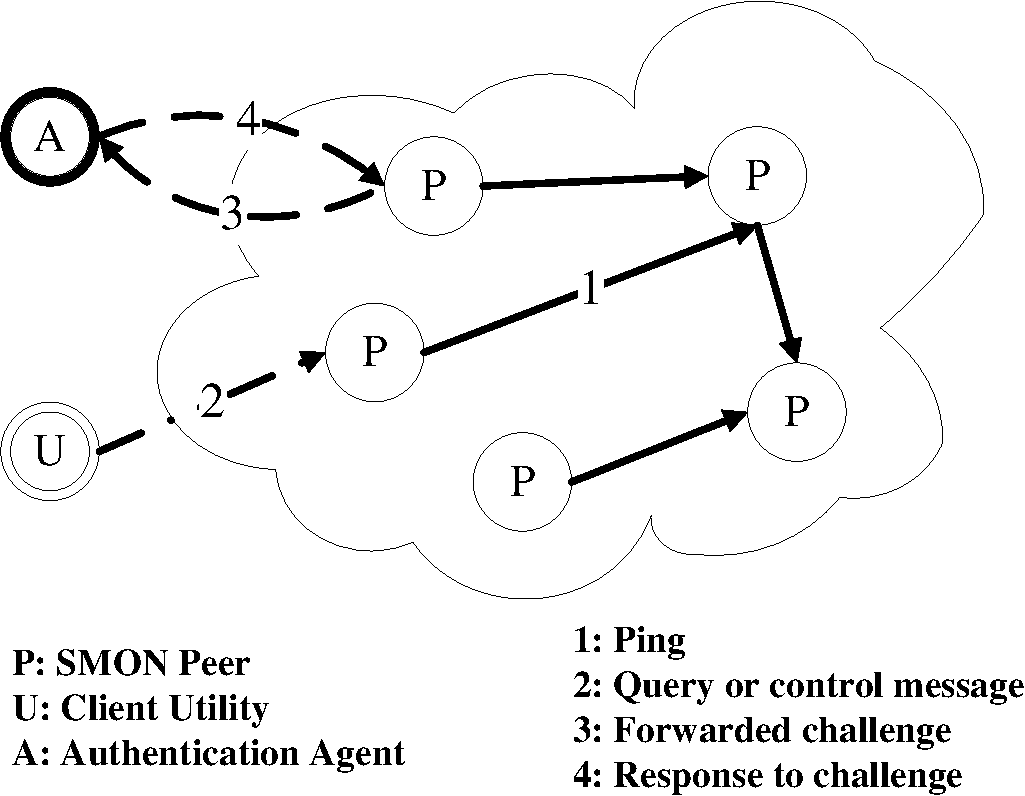
\includegraphics[width=3.0in]{smon_arch}
    \caption[SMON系统结构]{SMON系统结构。SMON系统由三部分构成,
    SMON管理节点、认证代理和
    客户端工具。SMON节点构成SMON系统的主要部分,认证代理协助SMON节点与远程
    机器认证,使用者通过客户端工具完成管理任务。}
    \label{fig:smon_arch}
  \end{minipage}
\end{figure}

SMON系统的体系结构如图~\ref{fig:smon_arch}所示,包含了三个部分:SMON节
点,认证代理和客户端工具。

SMON管理节点运行在分布式平台的一组机器上,每个节点都维护着完整的机器列
表,这个列表也称作是SMON节点的邻居列表。SMON节点相互探测并相互维护。
SMON节点定期从从邻居列表中选择一个节点,向它发一个ping消息,如果超时没
有收到回复的pong消息,那么这个SMON节点会试图向远程机器安装新的SMON节点,
如果远程机器已经安装有SMON节点,那么它将会试图恢复失败的SMON节点运行。
每个SMON节点都保存着自身的版本号,在用ping-pong消息相互探测过程中,会
顺便交换相互的版本号,低版本的SMON节点会将自身升级至高版本。

认证代理持有与分布式平台上的机器认证所需的认证信息(例如私钥)。当
SMON节点在远程机器上部署新的SMON节点,或者恢复失败的SMON节点时,需要首
先与远程机器认证并登陆,这一过程需要认证代理的协助。

用户使用客户端工具来管理一组分布式应用,这其中包括其它分布式管理系统。
通过这个办法,我们可以不断扩充SMON的管理能力。\note{这个说法需要斟酌。}

\subsection{自我管理设计}

我们分别描述SMON自我管理的三个方面:自我部署,自我更新和自我恢复。

\subsubsection*{自我部署}

% 一些啰嗦的表达方式:
% SMON可以自动部署至一组节点,一组分布式节点
% 相互探测,相互维护
% ping -> liveness

SMON可以自动将自己部署至分布式平台的一组目标机器上去。在最初状态时,所
有的目标机器上都没有被部署运行SMON节点。用户需要手动部署并启动一个SMON
节点。这个SMON节点会在邻居列表中随机选取一个机器,并在它上面部署第二个
SMON节点。新的SMON节点同样会在别的机器上部署SMON节点。当越来越多的SMON
节点被部署,自我部署过程会以幂指数速度增长。可以证明,以概率1,
所有可以连接的机器上都会被部署SMON节点~\cite{Eugster2004}。

详细来说,节点$P$会定期选择邻居列表里的一个机器$M$,并向它上发送SMON节
点探测消息(ping)。如果超时没有收到回应的pong消息,$P$就会在$M$上远程
部署一份SMON节点。它首先在认证代理的协助下(在\ref{subsec:security}节
中描述)认证并登陆进$M$,向$M$远程拷贝一份SMON的安装程序,并远程启动安
装程序。启动的安装程序首先检查自己的完整性(使用checksum校验和),以防
传输过程中产生错误,然后它会安装并启动SMON节点。

在上述过程运行的任何时刻,都有可能因为外界因素而产生错误(例如连接中断,
机器崩溃等)。如果有错误发生,$P$会直接放弃这次远程部署的任务。
epidemic算法能够保证,在未来,$M$会被另外一个SMON节点$P'$选中并部署
SMON节点。

自我部署过程中存在着竞争情形(race condition)。因为采用了epidemic算法,
多个SMON节点可能同时试图向同一个机器$M$部署SMON节点。这个问题不需要
SMON节点间直接协调便可以解决。不同SMON节点会将安装程序远程复制到$M$上的
不同目录,相互不会覆盖。如果有多份安装程序被同时启动,它们会使用操作系
统提供的同步机制(例如lock file),保证只有一份安装程序能够运行。因此,
只有第一个运行的安装程序能够完成安装。在解决这个竞争情形的过程中,引入
了一定的额外开销,会有多份安装程序被拷贝至同一台机器。这会浪费一部分存
储资源和网络带宽。经过实验测试,可以看出额外开销的数量在多大数机器上是
很小的。同时考虑到安装程序很小,只有122KB,因此可以认为额外开销的影响
不大。

自我部署过程何时结束是难以严格确定的。理想情况是,当所有目标节点上都被
部署并运行着SMON节点时,自我部署过程就可以称为结束了。但是,在分布式环
境下,某些节点可能会发生错误,或者不可连接,所以,实际情况下自我部署过
程很难达到理想情况。即使一个机器已经被部署了SMON节点,也有可能因为机器
或者网络错误的原因,造成某些SMON节点被关闭或者不可连接。因此,为了应对
分布式环境频繁发生的异常错误,每个SMON节点需要不断的监控其它节点。自我
部署何时结束是一个需要用户定义的问题。用户可以查询有多少机器已经部署且
运行着SMON节点,根据需要决定自我部署是否结束。

\subsubsection*{自我更新}

SMON可以将自己自动更新至新的新的版本。这个更新过程是在线进行的,用户不
需要因为更新而停止整个SMON系统。

每个SMON节点都有版本号,版本号被持久保存在每个SMON节点的配置文件中。
SMON节点会以epidemic方式交换相互的版本号。当发现相互的版本不同,版本低
的SMON节点会自动从高版本SMON节点那里获取新的安装程序,将自己更新至高版
本。为了把整个SMON系统更新至新版本,用户只需要更新一个SMON节点,整个
SMON系统会逐渐收敛至一个最终的版本。用户使用~\ref{subsec:client}节中描
述的客户端工具更新任何一个SMON节点。

存在着多个SMON节点向同一个版本SMON节点请求安装程序的可能,为了防止
瞬间拥挤(flash crowd)的冲击,节点会限制同时请求安装程序的数量。

\subsubsection*{自我恢复}

SMON系统可能遇到两种分布式环境中产生的错误:机器失败和网络分割。当一个
机器失败时,它上面运行的SMON节点也同时会被停止。SMON节点会尝试重新启动
失败的SMON节点,因此一旦失败的机器恢复,它上面的SMON节点会被重新启动。
同时启动多份SMON节点的实例是安全的,使用操作系统的同步机制,这等同于只
启动一个SMON实例。

网络分割也很容易应对。当网络分割发生时,SMON系统被分割为多个部分,每个
部分将会成为一个独立的小SMON系统,它们的状态,例如运行的SMON节点版本,
都将在各个部分内逐渐达成一致。当被分割的部分重新连接上时,不同部分的
节点会重新相互联系,从而整个系统的状态逐渐收敛。

\subsubsection*{自我管理小结}

将上述三个部分合并起来,就构成了SMON自我管理的内容。SMON节点通过相互探
测并执行相应的管理任务来达到整个SMON系统自我管理的目标。有两点值得说明。
第一、作为一个优化,SMON间使用ping-pong消息探测时,会顺便交换
(piggyback)它们的版本号。第二、如果节点$A$认为节点$B$失败,可能有两
个原因,或者$B$没有运行,或者$B$所在机器没有部署SMON节点。$A$会首先判
断远程机器上是否部署了SMON,并采取相应的步骤。

\subsubsection*{禁止、启动自我管理功能}

SMON的自我管理功能应该是能够被显式的禁止或者启动的。考虑如下场景:某个
研究人员使用SMON部署了一个分布式系统原型,在进行一些实验后,他决定停止
部署的分布式系统和SMON。如果SMON的自我管理功能没有被禁止,则整个SMON系
统不能够被停止。任何被用户停止的SMON节点,都很快会被其它SMON节点启动,
除非用户能够在一瞬间停止所有SMON节点,然而这在大规模分布式系统上是不可
能。

我们使用一个布尔变量\texttt{livetag}控制SMON节点的自我管理功能。如果它
的值是假,则节点停止定期探测其它节点的活动,因此整个系统停止了自我管理
的功能。这样,我们就能够逐一停止SMON节点,从而停止整个SMON系统了。

\texttt{livetag}变量有一个关联的版本号,每个SMON节点维护着变量的一个复
本。两个随机节点会定期交换\texttt{$<$livetag, version$>$}对,并且更新
\texttt{livetag}到最新的版本。需要注意到,节点交换\texttt{livetag}的行
为也是收到\texttt{livetag}值的控制的。当\texttt{livetag}值为假,节点不
会主动要求交换\texttt{$<$livetag, version$>$}对,但是任然会对交换消息
回复,这能够加快更新\texttt{livetag}的速度。

\subsection{安全机制}
\label{subsec:security}

SMON的安全机制需要保证如下两个目标:

\begin{itemize}

  \item 让节点能够自动与其它机器认证并登陆,从而节点能够自动安装新的
  SMON节点,或者远程恢复失败的SMON节点。

  \item 认证并加密SMON节点间的通信,不让系统被恶意利用,被用来部署
  恶意应用,例如botnet~\cite{botnet}。

\end{itemize}

我们首先叙述如何在Planet-Lab上设计达到上述两个目标的安全机制,并解释如
何在其它分布式计算平台上应用这个机制。Planet-Lab使用公钥系统来认证对系
统平台的访问。每个用户使用ssh访问他的slice~\footnote{Planet-Lab分配给
用户的一组分布式资源,表现形式是一组分布式虚拟机。}。用户私钥保存在
自己的机器上,对应的公钥被分发到用户slice的所有虚拟机里。

\begin{figure}
\centering
  \begin{minipage}{0.8\linewidth}
    \centering
    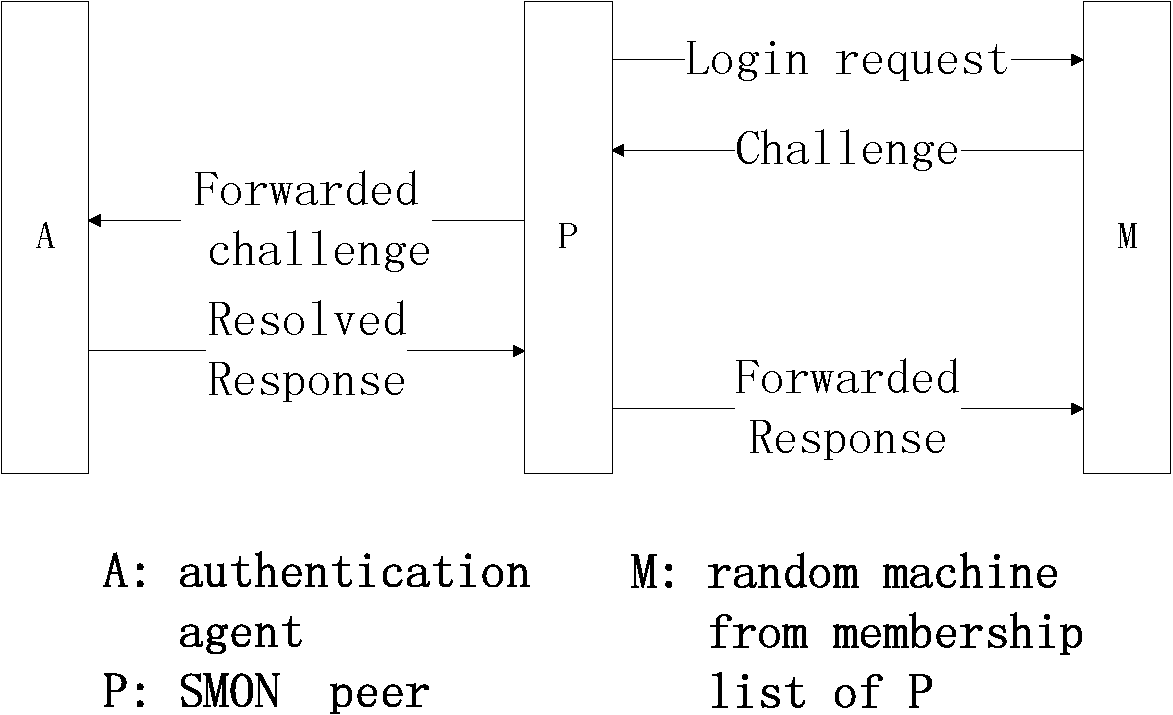
\includegraphics[width=3.0in]{auth}
    \caption{SMON节点在认证代理协助下与远程机器认证并登陆的过程。图显示
    了这一过程中三者的交互过程。}
    \label{fig:auth}
  \end{minipage}
\end{figure}

SMON引入了认证代理来协助节点自动与远程机器认证。认证代理持有用户私钥,
但私钥并不会被泄露。如图~\ref{fig:auth}所示,当SMON节点需要登陆到其它
机器上时,它首先连接远程机器的sshd服务器,并发送登陆请求。sshd服务器会
返回一个认证挑战密文,SMON节点没有用户私钥,无法求解对应的应答密文,它
会直接将挑战密文转发给认证代理,认证代理使用用户私钥求解得到应答密文,
并告诉SMON节点。SMON节点再将应答密文发送给sshd服务器。这样,SMON节点能
够登陆到用户slice内的任何一台机器上,并且用户私钥并未被泄露。

我们使用一个对称密钥$K_E$来认证和加密SMON节点之间、SMON节点和认证代理
之间的通信。$K_E$在SMON节点部署时一同被部署到各个机器上。由于部署的过
程中,通信是加密的,因此$K_E$不会被泄露。$K_E$也是可以安全保存在slice
内的机器上的,因为slice的虚拟机之间被很好的相互隔离。

用户应仔细评估并选择认证代理运行的机器,保证用户私钥的安全。认证代理不
必运行在用户slice内的某个机器上。如果SMON被部署的规模非常大,可以考虑
运行多份认证代理,提高认证的性能,同时有效的应对网络分割错误。SMON节点
可以在DNS服务器协助下~\cite{dns_akamai},将选择离自己最近的认证代理。

上面叙述的安全机制可以推广应用到其它分布式平台上,如果分布式平台满足下
面的两个假设:

\begin{itemize}
  \item 使用挑战-回应类型的认证方式,例如公钥认证机制,或密码认证机制。
  
  \item $K_E$可以安全的与SMON节点一起保存。
\end{itemize}

这两个假设可以被很多分布式平台满足,因此使用认证代理的安全机制可以被广
泛应用,例如Amazon EC2平台。在EC2平台上,用户使用ssh和他的私钥来访问一
组分布式虚拟机,这与Planet-Lab平台的情形非常类似。另外,私有集群,例如
学校或者企业内部的集群也可以应用认证代理安全机制。在这些集群上,一般都
安装使用Linux系统,访问集群内机器的方式也是ssh加用户私钥。虽然集群不一
定使用虚拟机隔离用户的资源,但是系统的用户都是非恶意的,因此$K_E$也可
以安全的保存在各个机器的本地文件系统上。另外,可以使用文件权限等工具,
进一步保护$K_E$的安全。

\subsection{邻居列表维护}

SMON系统的邻居列表有其自身的特点。一般来说,在其它分布式系统中,邻居列
表维护着一组正在运行的节点,而在SMON中,邻居列表是一组应该运行着SMON节
点的机器。SMON节点失败并不会影响邻居列表的内容。这个列表由SMON的用户指
定,并且通常不会发生改变。另外SMON系统要求,即使只有一个SMON节点在运行,
它也应该能够知道所有其它的目标管理机器。这意味着,任何SMON节点,都应该
能够知道整个目标管理机器列表。

在目前的设计使用了一个简单而实用的方案:每个SMON节点都维护着整个目标机
器列表的一个复本,列表通过压缩的方式存储在各个机器上。邻居列表有关联的
版本好,SMON节点会用epidemic的方式随机交换邻居列表的版本号,并更新旧版
本的邻居列表。通过改变邻居列表,用户可以改变SMON运行在哪些机器上。

这个邻居列表维护方案足够应用在上万规模的系统上。由于列表中只需要包含一
组节点的IP地址或者主机名称,一个简单的计算表明,用zip格式存储15000+规
模的节点列表,只需要大约100K的存储空间,这是可以接受的。

当邻居列表改变时,新添加的机器上会被自动部署新的SMON节点。从邻居列表中
删除的机器上的SMON节点也会在与其它节点交换邻居列表版本时,更新自己的邻
居列表,从而得知自己从列表中被删除。但是,它仍旧会不断的向新邻居列表中
的节点交换邻居列表版本与发送ping消息。这样,就帮助加快了散播邻居列表改
变的消息,同时帮助在新添加的机器上部署新的SMON节点。当大部分SMON节点更
新了它们的邻居列表时,SMON系统已经迁移到了一组新的机器上,位于列表中被
删除机器上的SMON节点将会很少收到来自其它节点的消息,这些SMON节点会在长
时间未收到消息的情况下,自动停止自己的运行。

\subsection{应用管理}

SMON可以管理若干个其它分布式应用。每个SMON节点负责部署和维护和它运行在
同一个机器内的分布式应用节点~\footnote{也就是分布式应用的进程}。每个应
用由它的名字所唯一标识。SMON节点会使用epidemic算法,定期与一个随机选择
的SMON节点交换它们管理的应用名称,如果发现一个新的未部署的应用,它会从
对方获取应用的安装程序,并在本机器部署安装新的应用。

应用被部署并启动后,会被同一机器上运行的SMON节点所监视并维护。应用可以
有两种状态,运行或停止。作为维护选项,用户可以指定应用应该出于哪一种状
态,可以有三种选择:

\begin{itemize}
  \item 始终在线(online):应用应始终在线,如果应用停止了,会被立即重
  新启动。

  \item 始终离线(offline):应用应始终离线。运行的应用会被停止。

  \item 忽略(ignore):仅在应用部署后启动应用,之后就不再监视应用的状
  态。
\end{itemize}

这三个维护选项指明了SMON应该如何维护一个被管理的分布式应用,这在应用被
部署时一同包含在配置文件中。用户也可以在应用部署后单独改变某个应用节点
的维护选项。SMON节点会定期向应用指定的一个中心节点报告应用的状态。当应
用的状态改变时,SMON会立即向那个中心节点报告这个变化。

显然,SMON提供的应用监测与维护语意是很基本的。对于一些情况,这样的管理
语意是足够的,例如维护一个需要长期运行的分布式应用,应用的节点需要尽可
能处在运行状态。由于这样的应用一般都经过一定测试,相对稳定,因此重启失
败的节点是恢复应用的直接手段。SMON提供的管理语意只考虑了应用是否运行,
而没有进一步监视应用是否运行在正确状态,包括应用的安全性与活性(safety
and liveness)。为了扩展管理语意,增加新的管理功能,用户可以在SMON上部
署其它的分布式应用管理系统。这在~\ref{sec:smon_app}节有进一步论述。

\subsection{客户端工具}
\label{subsec:client}

用户可以用SMON的客户端工具来控制SMON。客户端工具和SMON节点之间的通信受
到对称密钥$K_E$认证和加密保护。为了部署一个新SMON系统,客户端工具会在
用户指定的一台机器上远程部署并启动一个SMON节点,之后,SMON会自动将自己
部署到用户指定的邻居列表内的机器上去。为了更新SMON系统,客户端工具将自
己模拟为一个SMON节点,并和任意一个SMON节点发送交换版本号消息,从而,那
个SMON节点会从客户端工具获取新的SMON安装程序,并更新自身,接下来,整个
SMON系统都会得到更新。类似的,用户可以使用客户端工具来部署新的分布式应
用程序,更新邻居列表,禁止与启动SMON的自我管理功能,等等。SMON系统的最
新版本号,以及邻居列表、\texttt{livetag}的最新版本号也由客户端工具维护,
集中保存在用户的机器上。最后,SMON节点实现了一组RPC,用户可以使用客户
端工具调用远程SMON的RPC,查询SMON节点的状态、应用的状态,以及管理分布
式应用,改变应用某个节点的维护选项。

\section{实现细节}
\label{sec:smon_impl}

我们针对Planet-Lab平台设计了SMON原型系统。Planet-Lab是一个全球范围的分
布式计算平台,它包含了超过400个站点,规模超过800个节点。使用
Planet-Lab的用户需要注册一个账号,并将账号与一个或多个slice相关联。
slice是Planet-Lab分配分布式资源的方式,一个slice对应分布在不同节点上的
一组虚拟机。用户可以使用ssh以公钥认证的方式登录他的slice里的机器。

我们使用Python语言实现SMON系统原型。最终的SMON节点安装程序大约122KB大
小,包括超过1000行代码。

我们使用单独的线程实现SMON节点运行时的epidemic活动。包括一个探测并维护
其它节点,实现自我管理功能的线程,一个更新邻居节点线程,一个更新
\texttt{livetag}的线程。对每一个应用,我们启动一个单独的管理与维护线程。

\begin{table*}
\small
\centering
\caption{SMON节点通信使用的RPC}
\label{fig:smon_rpc}
\begin{tabular}{|l|p{7cm}|}

\hline
\textbf{RPC} & \textbf{功能描述} \\

\hline
\texttt{ping(ver)} & Call with local SMON peer's version and
return remote peer's version.\\

\hline
\texttt{retrieve\_peer(ver)} & Retrieve installation package
of SMON peer with specified version.\\

\hline
\texttt{exchange\_livetag(tag, ver)} & Call with local
$<$livetag, version$>$, and return remote peer's $<$livetag,
version$>$.\\

\hline
\texttt{exchange\_member(ver)} & Call with local membership
list version and return remote peer's membership list.\\

\hline
\texttt{retreive\_member(ver)} & Retrive membership list of
specified version.\\

\hline
\texttt{exchange\_app(app\_name)} & Call with an application
name, return true if remote peer has installed the
application.\\

\hline
\texttt{retrieve\_app(app\_name)} & Retrieve installation package
of an application with specified name.\\

\hline
\texttt{resolve\_challenge(challenge)} & Return the response
to an authentication challenge.\\

\hline
\texttt{set\_app\_status(app\_name, status)} & Set application status (online,
offline, ignore).\\

\hline
\texttt{get\_app\_status()} & Get application status. \\

\hline

\end{tabular}
\end{table*}


SMON节点间的通信使用RPC机制实现,总结在表~\ref{fig:smon_rpc}中。

SMON节点通过spawn一个ssh/scp进程来远程复制安装程序或者执行命令。我们使
用修改的\texttt{ssh-agent}将ssh认证时的挑战密文转发给认证代理,实现自
动认证的过程。认证代理实现了RPC接口\texttt{resolve\_challenge},其输入
参数是认证的挑战密文,返回对应的应答密文。

SMON节点运行时的参数保存在一个配置文件中。包括连续epdemic活动之间的时
间间隔,SMON节点和邻居列表的版本号,$<$\texttt{livetag, version}$>$对,
以及认证代理的地址。每个应用也可以指定应用状态变化时目标报告节点的地址。
配置文件用SQLite数据库实现,保证数据不会在机器崩溃时丢失。配置文件由
SMON节点与应用的安装程序更新。邻居列表单独保存在一个压缩文件中。


\section{应用方式}
\label{sec:smon_app}
plush

d3s

scalpel

\section{性能评价}
\label{sec:smon_eval}

我们在Planet-Lab平台上评测了SMON系统的性能指标。Planet-Lab是一个全球范
围的分布式计算平台,它包含了超过400的站点,规模超过800个节点。具体的说,
通过评测,我们能够看出,SMON系统的自我部署过程是有效的,并且有很好的可
扩展性。在自我部署过程中由于竞争情形引发的额外开销是足够小的,另外,
SMON系统的自我管理功能能够很快的在禁止和启动状态间转换。

\begin{figure}
\centering
  \begin{minipage}{0.8\linewidth}
    \centering
    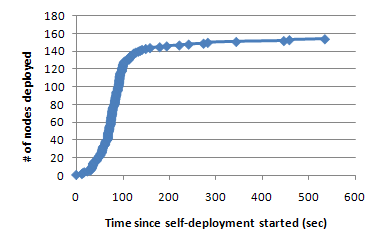
\includegraphics[scale=0.618]{self-deploy.png}
    \caption{SMON在159个Planet-Lab机器上自我部署的进度}
    \label{fig:self-deploy}
  \end{minipage}
\end{figure}

首先,我们试图让SMON在159台Planet-Lab节点上完成自我部署,并观测部署性
能。我们在随机选取的一个Planet-Lab节点上,部署并启动了一个SMON节点,自
我部署过程开始。在目前设计中,SMON节点每隔5秒种,随机探测其它1个节点。
我们最终收集到154个节点上的数据,其它5个节点由于连接不上,因此它们的结
果不能取得。这种情况在大规模分布式系统中是很常见的。图~
\ref{fig:self-deploy}总结了部署过程的进度。我们可以看出,90\%(143个)
的节点,在149秒内被成功的部署了SMON节点。部署时间的中值是93秒,最后一
个节点被部署的时间是533秒。图~\ref{fig:self-deploy}中的“尾巴”是由于
两个原因造成的,一些机器由于负载太重,因此反应迟钝,另外连接至一些机器
的网络速度太慢,因此部署的速度比较慢。

\note{为什么曲线是先快后慢}

\note{overhead的模型?}

\begin{figure}
\centering
  \begin{minipage}{0.8\linewidth}
    \centering
    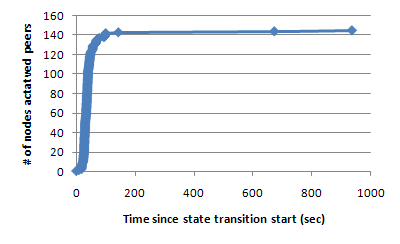
\includegraphics[scale=0.618]{state-trans.png}
    \caption{SMON的自我管理功能从禁止到启动过程的进度}
    \label{fig:state-transition}
  \end{minipage}
\end{figure}

SMON系统能够在活跃和非活跃状态间转换是非常重要的。我们在这里评测它状态
转换的性能。我们让在159个Planet-Lab节点上部署的SMON系统,从非活跃状态
变成活跃状态。图~\ref{fig:state-transition}总结了转换的进度。对于90\%
的节点来说,状态在143秒后成功的转换,而状态转换的中值是37秒。可以看出,
状态转换过程是非常快的。

\begin{figure}
\centering
  \begin{minipage}{0.8\linewidth}
    \centering
    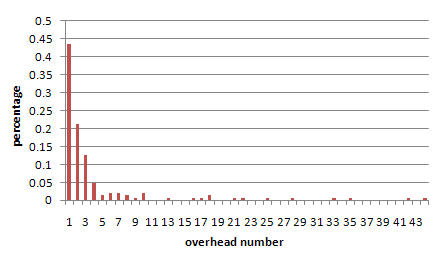
\includegraphics[scale=0.5]{overhead.png}
    \caption{为了解决自我部署过程中的竞争情形而产生的额外开销分布。}
    \label{fig:overhead}
  \end{minipage}
\end{figure}

在自我部署过程中,存在着竞争情形,也就是多个SMON节点可能会在同一个机器
上部署新的SMON节点,这将引发额外开销。这个开销将会浪费网络和节点的存储
资源。我们计算了在每个机器上,发生的同时部署个数。结果显示在图~
\ref{fig:overhead}中。可以看出,有43.71\%的机器,只被部署了一次,对于
大部分机器,部署次数都在10以内,这样的机器覆盖了机器总数的92.04\%。平
均来说,每个机器被部署了4.30次,而部署次数在10以内的机器,它们的平均部
署次数是2.31。这样的结果表明,为解决竞争情形而引发的额外开销是可以接受
的。

\begin{table}
\centering
  \begin{minipage}{0.8\linewidth}
    \centering
    \caption{在不同的规模SMON自我部署性能比较}
    \label{fig:scalability}
    \begin{tabular}{|l|c|c|}
    \hline
           & 24 nodes & 159 nodes\\
    \hline
    median & 58 sec & 82 sec \\
    \hline
    90\%完成 & 85 sec & 149 sec\\
    \hline
    最终完成 & 103 sec & 533 sec\\
    \hline
    \end{tabular}
  \end{minipage}
\end{table}

为了评测自我部署过程的可扩展性,我们比较了在不同规模下部署SMON系统的性
能。我们在另外的24个节点上部署了新的SMON系统。表~\ref{fig:scalability}
总结并对比了在两个规模下的部署性能。从表中我们可以看出,两个系统规模的
比例是6.6(159/24),但是90\%进度的部署时间比例只有1.75(149/85),而
部署时间中值的比例是1.41(82/58)。可以看出,SMON系统具有良好的扩展性。

\section{相关工作}
\label{sec:smon_related}

\section{本章小结}
\label{sec:smon_conclusion}

% vim:textwidth=70
\chapter{自动推断系统层次结构任务模型的方法}
\label{chap:scalpel}

\section{本章引言}

随着Internet服务逐渐渗入人们日常的生产生活,它们的可靠性也变的越来
越重要。系统设计实现上的缺陷,一直伴随着这些服务而生,导致服务性能下降,
甚至彻底中断运行。在诸多的软件缺陷(bug)中,那些最难找到和解决的是让
系统仍然运行,但是却偏离了系统期望行为的缺陷。这些缺陷的根本原因,隐藏
在复杂甚至是混乱的应用逻辑中,因此寻找并分析这些缺陷变的异常困难。

支撑Internet服务的系统本质上就非常复杂,这更增加了分析理解系统异常行为
的难度。这些系统通常使用了分层的体系结构,将其功能抽象表达为不同的层次
结构。\note{high degrees of concurrency}。系统在运行时,处理着许多用户
层次的\emph{任务},例如用户请求,任务被分成许多阶段执行,不同的阶段
被分布在多个机器、进程和线程上执行,使用事件或者异步消息作为通知机制。
验证单独每个任务的行为,是一件具有挑战性的问题,因为开发人员需要重构出
任务的执行流,将任务执行过程中的各个阶段重新连接起来。

从概念上说,开发人员可以把任务执行表示为\emph{层次结构的任务模型},
这与系统的分层体系结构设计一致。不同层次的任务表示在不同阶段不同模块执
行的一段执行过程。高层任务的执行被分为若干低层子任务。\note{pacifica
example}。基于任务模型,开发人员可以更好的理解系统模块间的结构,以及不
同模块间的依赖关系,并验证出于不同层次任务的行为。

然而,目前的\note{工具}需要开发人员手动标注任务模型。例如,
Pip~\cite{pip}要求开发人员将系统预期行为,用“期望(expectations)”的
形式表达,“期望”表达了系统正确执行时的任务模型,包括对执行时资源使用
的约束。通过对比期望与实际执行的区别,可以验证系统运行时行为。写出一个
全面表达系统高层设计与底层实现的期望是非常困难的并容易出错的事情,特别
对那些正在快速发展中的系统。基于执行路径的工具,例如
Magpie~\cite{magpie},可以从单独的运行事件trace推断每个请求的执行路径,
但是它仅可以处理的一组事前确定的事件,并且需要开发人员指定任务的边界与
关联条件。

本文的目的是探索不需要人工帮助,自动推断层次结构任务模型的方法。开发人
员不需要手动标注源代码来指定任务边界,并却任务的层次结构也应该能够自动
推断得到。这样,开发人员和系统管理员就可以利用得到的任务模型,以可视化
的形式表现系统设计和实现,也可以将任务模型作为输入,使用其它工具调试或
验证系统设计。

设计一个自动任务模型的推断工具面临如下几个挑战性问题。首先,应该能够确
认合适的任务边界,这一过程应该只基于对系统执行过程的监视,而不需要开发
人员显示的标注。其次,必须能够正确的关联任务之间依赖关系。特别是,必须
能够辨别任务之间因为共享资源(例如,共享队列、锁等)而产生的依赖关系。
最后,应该能够自动恢复任务的层次结构。任务由许多或者顺序或者并行的子任
务构成。考虑到复杂系统中任务执行的非确定性,确定它们的依赖关系与层次结
构并不容易。

在本文中,我们描述了如何自动推断复杂系统层次结构任务模型的方法,并实现
了一个原型系统Scalpel。我们通过使用插装(instrument)技术来透明的观测
系统运行,获取系统运行过程的trace,包括用户和系统函数调用的过程。自动
推断方法使用trace作为输入,自下而上(bottom-up)的推断系统层次结构任务
模型,推断的过程分为三步,分别对应上面提到的三个挑战性问题。

首先,我们将运行过程分为一个个叶子任务,它们是层次结构任务模型中最基本
的任务。叶子任务的边界对应执行的同步点(synchronization point)。在同
步点,线程或进程相互同步从而具有依赖关系,因此同步点是推断任务边界的一
个合理启发点(heuristic)。

其次,我们按照运行时的因果依赖关系,将叶子任务用有向边连接,形成一个因
果关系图。叶子任务的因果依赖关系由任务运行时的执行顺序推断得到。

最后,我们在任务关系图上,推断出层次结构。每一个层次,大致对应系统设计
与实现上的一个层次。我们使用聚类算法寻找任务关系图上重复出现的模式(就
是频繁子图),以此为依据确认高层任务与构成它的子任务。通过递归的使用聚
类算法,我们能够进一步寻找更高层次的任务。

\note{prelimianry experience}

\note{文章安排}


\section{设计}

本章叙述推断方法设计,以及它的原型实现\pozhehao{}Scalpel。

\subsection{收集系统运行trace}
收集什么

全序关系?



\subsection{确定叶子任务}

在系统执行trace的基础上,我们首先需要确定叶子任务的边界。Scalpel使用
\emph{同步点}作为启发点定义任务边界。同步点是两个线程同步相互执行,从
而具有执行顺序关系的地方。在同步点,线程可能因为互斥或者相互协同而具有
顺序关系,前者的例子是线程使用锁同步对共享资源的访问,后者的例子是线程
等待另外一个线程的信号消息。

我们定义两个相继的同步点之间的执行为一个叶子任务。采用这个定义的原因是,
首先两个同步点之间的一段执行是相对独立,并且自包含的。因此,它们合理的
成为任务模型中最小粒度的一段执行,也是叶子任务的一个自然定义。另外,因
为采用了同步点定义叶子任务的边界,叶子任务之间的依赖关系也只发生在边界
之间。

Scalpel通过插装系统函数库中的同步原语(锁、信号、事件等)与socket操作
\footnote{我们认为通信也是一种同步操作。}获得相关的trace。在实际系统中
的应用经验表明,插装这些系统操作是足够的。如果应用系统使用spin-lock或
者lock-free的数据结构,则仅插装系统调用是不够的。这时Scalpel会丢失一些
同步点从而使任务模型粒度更粗。手工标注可以解决这个问题,但是整个推断方
法不再是全自动的。鉴于多数实际系统还是采用系统调用进行同步,我们将这个
问题留作将来的工作。

\subsection{任务因果关系图}

为了推断任务的层次结构,我们首先要连接叶子任务直接的依赖关系。我们使用
因果关系图。这个图中,节点表示叶子任务,有向边表示叶子任务直接的依赖关
系。\note{For example, in PacificA...}。

Scalpel使用执行顺序关系推断任务的因果依赖关系,这包括同一线程内顺序执
行的两个叶子任务,以及因为同步而依次执行的叶子任务。我们需要将“假”的
因果依赖关系区别并去除。一个“真”的依赖关系的例子是,一个从队列里取出
并处理事件的任务,在因果关系上依赖于产生那个事件并将其加入队列的任务。
另一方面,如果两个线程使用互斥锁同步对共享资源(例如I/O)的访问,虽然
它们的行为在表面上也构成因果依赖关系,但实际上,任务直接并不相互依赖,
其执行的顺序有调度器随机决定。因此,我们将互斥排除在因果关系之外。

Scalpel使用若干启发点分辨真的因果依赖关系。如果系统使用操作系统提供的
队列(例如I/O completion ports),或者通知机制(例如event),则可以使
用同步操作使用的句柄(保存在插装得到的trace中,是同步操作的参数),将
生产线程与消费线程联系起来。对于操作系统的互斥锁(mutex)与信号量
(semaphore)对象,它们通常被用来同步线程对共享资源的访问,因此不认为
它们构成因果依赖关系。

\note{match socket}


\subsection{推断任务层次结构}

递归寻找frequent subgraph

具体做法

子图相似度定义

具体算法(伪代码)

\subsection{实现}

a

\section{讨论}

a

\section{验证推断方法}

iocp, event, mutex

\section{应用实例}

apache, sqlite

pacifica

// statistics

\section{性能评测}

overhead, script run time, 


\section{相关工作}

a

\section{本章小结}

a


% vim:textwidth=70
\chapter{基于日志的任务层次结构推断方法}
% XXX: model may not appropriate because no dependency
\label{chap:logmining}

\section{本章引言}

随着云计算逐渐影响人们的生活,分布式系统变的越来越重要,成了Internet应
用的关键组成部分~\cite{gfs, mapreduce, bigtable, dynamo}。分布式系统运
行在多台机器上,充分发掘并调度机器资源,以提供高吞吐率、低延迟的服务,
同时,还要处理各种不同类型的系统失败事件(failure)。由于系统规模庞大,
并且有严格的服务质量要求,设计与实现这类分布式系统不可避免的会产生错误
(bug),从而使系统表现出未预期的行为。系统错误的根本原因通常隐含在复
杂的应用逻辑之下,找到这些错误通常会花费很长时间。

理解分布式系统的运行时行为是验证系统设计、发现系统逻辑与性能问题、解决
系统实现错误的关键。然而,即使对系统的实现者来说,充分理解系统逻辑也不
是一件轻而易举的事情。这是因为,系统设计非常复杂,它的运行时行为多种多
样。再者,系统通常由一组程序员共同开发,并且在不停的演变至新的版本。进
一步说,分布式系统通常会使用分层的设计模式,用户请求由不同层次的模块处
理。上层模块中的某个函数,会由下层模块的多个函数一起完成,其完成方式,
可能是顺序的,也可能是并行的,跨越多个机器、进程与线程。以上这些状况,
都增加了理解系统运行时行为的困难。

已有的方法表明,用分层的任务模型去表达系统行为,可以很好的帮助程序员理
解与验证系统。例如,Pip~\cite{pip}允许程序员定义可嵌套的任务流,并定义
“期望”,来发现异常。用这个方法,程序员能够定义并验证系统特定层次的特
性。这种方法被证明能够很有效的发现系统错误与性能问题。我们之前的工作
Scalpel~\cite{scalpel}进一步发展了一种方法,能够从底层系统调用trace中,
自动推断任务模型,从而避免了手动定义任务结构的工作。初步的结果表明,从
操作系统层次的同步操作,我们能够推断出合理的表达上层语意的层次结构任务
模型。利用得到的模型,我们能够帮助程序员快速的发现并解决系统性能问题。

我们最终的目标是设计一个完全不需要或尽可能少需要人工标注的工具,来自动
提取系统的分层任务模型,帮助程序员、测试人员和系统管理员理解系统运行时
行为。基于之前的工作,在本文中,我们重点研究了如何利用应用日志(log)
来推断任务层次结构。其基本原理是,相比底层trace,应用日志包含了更多的
应用层任务流的语意。日志是由系统开发人员创建的,因此它们包含了关键的系
统状态和事件信息,例如,用户层任务的开始和结束,处理用户请求的关键步骤
等等。利用这些信息,可以帮助我们推断用户层语意,而这些很难从系统调用
trace中得到。

使用日志推断任务层次结构需要解决两个问题。第一、日志通常是非结构化的,
我们需要从中提取出和任务相关的信息。第二、推断任务之间的层次关系,从而
可以将系统活动分为层次结构的任务实例。

我们的解决方法是,首先,通过使用一组简单的启发,尽可能提取出日志中的任
务信息,包括任务的名称与ID。接着,通过推断任务ID的变化,推断任务的层次
关系。例如,我们可以在日志中发现这样的模式“request=R1,
operation=op1\yuanquan{a}\ldots \ldots request=R1,
operation=op2\yuanquan{b}\ldots \ldots request=R2,
operation=op3\yuanquan{c}”。request、operation是任务的名称,它们的值
表示相应任务ID。通过观察request任务ID的变化,我们可以推断R1任务的边界
在\yuanquan{a}处开始,在\yuanquan{c}之前结束,之间的日志条目都属于任务
R1,描述它的执行过程。进一步,任务是有层次关系的,同一个日志条目,可能
属于多个任务,通过观察多个任务ID的变化关系,我们可以推断不同任务之间的
层次关系。例如,同时考虑任务request和operation,我们发现,\yuanquan{a}
\yuanquan{c}之间的任务,同属于一个request任务R1,但是分属于不同的
operation任务,从而我们推断,request和operation任务之间,有层次嵌套关
系。通过对日志中所有的任务标识进行提取和推断,我们可以有效的推断出任务
之间的层次关系来。

我们实现了基于日志的任务层次结构推断工具,并使用它分析一个分布式存储系
统ChunkFS。ChunkFS是一个类似GFS~\cite{gfs}的分布式文件系统。我们的工具
能够推断出合乎逻辑的任务层次关系。应用得到的层次关系,能够帮助我们理解
ChunkFS的实际运行过程,并解决了ChunkFS中的一个性能问题。经验表明,系统
日志能够很好的反映出上层语意,我们的工具可以帮助理解系统设计和运行时行
为。

% XXX:文章组织

\section{推断方法设计}

图表 1是推断工具设计概要。我们首先从无结构的系统日志文本中提取出任务信
息,并用(key, value)形式表示。key是任务名称,value是任务ID。之后,我
们推断key也就是任务之间的层次关系。我们将层次关系转换为任务模型,并利
用任务模型分析系统动态行为。

\subsection{提取任务信息}

日志包含了大量系统活动信息。我们需要从无结构日志文本中提取描述任务行为
与状态的信息。日志中包含的信息通常可以表达成为(key,value)对的形式。
我们首先提取出所有的(key,value)对,并从中筛选出key是任务名称的(key,
value)对。我们使用的方法适用于ChunkFS的日志,其原理可以推广应用至其它
类型的日志。

图表 1顶部是一个ChunkFS日志的例子。不同系统的日志格式也不
相同,我们的日志格式是一个典型代表。日志头的部分记录了日志的级别、时间
、类别,紧接着是所在文件、函数和行号,最后是进程号、线程号。日志头是固
定格式的。日志的后半部分,包含在Notes域里。它是程序员记录的系统状态,
包含了文字描述与数值表达的系统状态参数。任务信息通常都记录在这里。

由于
Notes中的内容是无结构的,因此从中提取出(key,value)信息并不容易。我
们观察到,(key,value)在日志中通常被写成key SEP1 value SEP2的形式。
其中,SEP1是key和value的分隔符,SEP2是两个(key,value)之间的分隔符。
SEP1和SEP2的选择很多,可能是空格、逗号,分号等多种形式。从日志中,并不
容易确定哪个单词是key,因为key和文字描述中的单词可能是相同的形式,例如
POSTED: 和opId:。

我们使用了一种新颖的办法提取(key,value)信息。基于
对日志的观察,我们发现,value部分的格式是有限的,通常包括整数、十六进
制数和GUID,很容易使用正则表达式来匹配。一旦找到value部分,我们可以在
文字中向前跳过分隔符SEP1,遇到的第一个单词就是对应的key。

在少数情况下,
value也可能是一个单词。但是目前我们只提取value为数值格式的(key,value)
对。这是因为,1)文字形式的value只是对某个状态的简单描述,对于推断任务
层次关系用处不大,2)由于SEP1和SEP2可能是空格,在这种情况下,文字形式
的value,会和key、其它文字混淆,无法区分。

对提取出的(key,value)检查
时,我们发现,由于程序员创建日志时未对key的命名作严格约定,会产生下面
问题:1)同一个key会有多个别名,2)不同的key可能使用相同的名字(key冲
突)。我们使用命名映射同时解决了这两个问题。在解析完一个日志条目后,会
依据映射规则,把某些key转换为新名字。

映射规则的形式如(FileX, FuncY,
key)(newkey),表示如果一个日志条目的所属文件、函数是FileX、FuncY,
那么将这个条目中的key转换为新的名字newkey。FileX, FuncY可以使用正规表
达式。这样,key别名可以用(*, *, alias)(key)映射规则解决,而key冲
突问题可以用(FileX, FuncY, conflict key)(newkey)映射规则解决,从
实际经验看,通常只需要指明FuncY就可以解决冲突。

通常来说,并不是每个提取出的(key,value)对都描述任务信息,例如key是
error时,它描述的是某个任务执行的错误码。我们需要筛选出key表述任务名称
的(key,value)对来,这有两种情况。第一,key直接就是任务的名称,例如
Session。第二,key是与任务一一对应的请求或数据。例如key是requestID或
eventID,表示目前正在处理的请求/事件是requestID,requestID与任务有一一
对应关系,因此可以用 requestID代表正在处理它的任务。正确的判别key是否
描述任务信息,需要理解 key的语意。我们采用了半自动的方法来解决这一问题,
首先,使用正则表达式,筛选掉肯定不表达任务信息的key,例如*size*,
*err*, *offset*,接下来,请系统开发人员选出正确的key集合。采用这种方法,
我们能够筛选掉大部分的不表达任务信息的key,从而降低了开发人员的工作。

\subsection{推断任务层次关系}

实际系统中的任务是有层次关系的,表现为不同的任务之间嵌套关系。一个高层
任务的执行,会被分解成为若干个低层任务。我们将任务之间的这种层次关系用
>表示,例如keyS>keyP。keyS、keyP是任务名称。经过提取任务信息步骤,我
们得到顺序的(key,value)任务信息序列,接下来,我们推断这个序列中key
之间的关系,并输出一组(keyS,keyP,R)三元组,表示keyS>keyP,且分数
是R。

我们首先给出一个(key,value)序列的例子,如图表 2,以利于读者理解推断
算法。图表 2中,摘取了从ChunkFS客户端日志中提取的任务序列片段,它的意
义是:在任务Session s1中,处理了某个客户端命令,对stream x1进行操作,
这些操作分成若干opId子任务执行,在opId 1中,首先进行了stream层次的操作,
例如打开、创建一个stream,之后,opId 2/3对stream的不同chunk进行操作。
 
图表 2 任务信息(key, value)序列示例

我们使用如下两条规则从(key, value)序列中推断任务之间的层次关系,它们是
两个任务有>关系的充要条件。

规则一:如果keyS$>$keyP,那么在(key, value)序列中,keyS的第一次
出现早于keyP的第一次出现。

规则二:如果keyS$>$keyP,那么keyS的值域与keyP的值域,有严格的一对多关系,
也就是一个子任务,只能属于一个父任务。

通过规则一,我们可以得到所有任务之间可能的层次关系,通过规则二,我们将
规则一得到的错误结果筛去。

推断算法详细描述如下。算法扫描(key,value)序列,并顺序更新三个数据结
构。第一,每个key最新的value。第二,一个key数组,维护key之间的偏序关系,
与规则一对应。数组中任何一个key,都是它后面key的潜在父任务。算法若遇到
(key,value)对,其key不在key数组中,则将它加入数组。第三,任意两个
key它们值域(value)的对应关系,与规则二对应。对每个扫描到的
(keyP,valueP),将(valueS,valueP)加入(keyS,keyP)的值域对应关系
(用一个数组维护),keyS是key数组中所有keyP前面的任务(即keyP的潜在父
任务),valueS、valueP是keyS、keyP的当前值。

这样,当扫描完(key,value)序列所有数据后,我们得到每一对(keyS,keyP)
的值域对应关系数组。应用规则二,判断是否keyS和keyP的值域有严格的一对多
关系,如果满足条件,那么使用(valueS,valueP)数组的长度,作为(keyS,
keyP)的分数R。

对图表 2中的例子,应用上面描述的算法,可以得出,StreamID>ChunkID,分
数为4,Session>opId,分数为6。Session和StreamID之间没有层次关系,因为
多个Session可能对应相同的StreamID。类似的(Session,ChunkID),(opId,
StreamID)和(opId, ChunkID)也没有层次关系。

我们认识到,正确判断两个key是否有层次关系依赖于是否有足够多的数据,使
得不存在层次关系的key使用规则二被筛选掉。通常情况下,系统日志都足够大,
包含充分的数据,能够正确判断key的层次关系。

\subsection{构建分层任务模型}

经过上一步,我们得到了任务两两之间层次关系。将所有这些关系联系起来,得
到了所有任务之间的偏序关系,可以用一颗或多颗树来表达得到的偏序关系。每
一颗树都是一个层次结构的任务模型。在树中,每个节点都是一个任务,在实际
执行过程中,这个任务的执行过程包含若干它的子任务。程序员可以选择任意一
个任务模型对系统进行分析。为表示清晰起见,若原有任务模型的树根是
RootTask,我们增加一个新的节点Runtime,令它为RootTask的父节点,表示系
统运行时行为,由若干RootTask构成。

例如,对图表 2,可以得到两个任务模型,RuntimeSession, SessionopId
和RuntimeStreamID, StreamIDChunkID。

我们将任务模型应用在系统日志上,将系统运行时行为分为有层次的任务实例,
每个实例都由一组系统日志构成,描述一段时间内的系统活动。系统行为首先从
任务模型的树根开始,分为高层任务实例。每个任务实例开始于任务ID被赋予一
个新的值,结束于任务ID被赋予另外一个值之前。在每个任务实例内部,被递归
的分为更低层的任务实例。

对于图表 2中的例子,我们应用RuntimeSession, SessionopId任务模型,
得到图表 3中的有层次的任务实例。

我们认识到,系统运行时包含若干线程,因此“推断任务层次关系”与“构建分
层任务模型”两个步骤都是对每个线程分别操作,并使用基于数值的join操作
[7]将不同线程的任务联系在一起。

\section{应用}

在这一节,我们报告使用第3节中的推断工具,从ChunkFS日志中提取任务模型,
并应用模型理解ChunkFS动态行为。同时,我们也描述了,如何利用任务模型,
解决系统的性能问题。

\subsection{理解系统运行时行为}

ChunkFS是一个分布式存储系统,它类似于GFS。ChunkFS由一个master和若干个
chunkserver构成。在ChunkFS中,数据被组织成一个个stream,对应GFS中的文
件概念。每个stream,由若干chunk构成。每个stream和chunk都有唯一的GUID标
识。我们在集群环境下部署一个ChunkFS实例,包含一个master,若干个
chunkserver。接下来,向ChunkFS中随机的上传了若干文件,在上传命令之间,
还随机插入了若干查询命令,获取已上传文件的属性。

% 若干文件?

首先分析ChunkFS客户端行为。我们发现ChunkFS客户端运行时有两类线程:一个
client线程和若干个worker线程。Client线程的任务模型是Runtime$>$Session,
Session$>$opId,worker线程的任务模型是Runtime$>$opId。

Client线程接收用户命令,每个用户命令,由一个新的session任务执行,
session任务被分为若干步骤,每一步是一个opId任务。在一个opId中,会发起
一到多个RPC调用,client线程并不直接调用RPC命令,而是将这个调用放入一个
RPC队列。Worker线程从RPC队列中取出RPC命令,并调用它们。当RPC命令返回时,
worker线程向client线程报告RPC调用的结果。对worker线程来说,它们的行为
被分为若干opId任务。Client线程和worker线程通过相同的opId联系到一起。

我们详细的观察了上传文件至ChunkFS的过程,如图表 4所示。在客户端,创建
新stream命令涉及一个session和4个opId,有6个RPC调用,具体过程是(create
stream),(append stream,append chunk),(append chunk),(append
chunk,seal the chunk)。每个括号代表一个opId任务,括号内是RPC调用。由
于文件小于chunk大小的最大值,创建的stream只有一个chunk,其内容由3次
append chunk RPC调用写入。在最后一次append chunk RPC调用之后,chunk被
封装,即seal chunk RPC调用,之后,chunk不能再被写入或追加(append)。

 
图表 4 创建一个Stream操作,ChunkFS客户端运行时行为。每个圆圈代表一个
opId任务,整个四个圆圈代表一个Session任务


我们同时观察在primary chunkserver端的运行时行为。Chunkserver端运行时包
括若干线程,其任务模型是RuntimeChunkID。具体的,创建一个
stream,Chunksever会接到5个RPC调用,如图表 5所示,分别是create chunk,
3个append chunk和seal chunk。可观察到的chunkserver行为的粒度被限制在对
chunk操作的级别(ChunkID任务),因此5个RPC处理被认为是同一个任务实例。

 
图表 5创建一个Stream操作,ChunkFS Chunkserver运行时行为。5个RPC被当作
一个ChunkID任务,因为它们都对同一个Chuck进行操作。


经验:使用任务模型,我们可以有效的把系统运行时活动分为不同层次的任务实
例,有效的理解系统行为。任务模型实际上是隐含在系统设计中的,利用任务模
型从上至下的分解系统活动是有效的。

我们注意到,使用任务模型,也会产生一些不精确的地方。第一、任务边界可能
会有位移。通常任务都有一个初始化步骤,在这期间,任务标识可能还没有产生,
因此使用任务标识的变化来确定任务边界,会把初始化部分划分到上一个任务的
尾部。考虑到初始化部分通常是比较固定的若干步骤,可以对任务边界增加一个
修正量,解决这一问题。第二、任务的粒度依赖与任务模型的精确程度。例如在
先前的chunkserver例子中,5个RPC是五个不同的任务,但是由于使用Runtime
ChunkID模型,且这5个RPC处理是连续的,所以会被认为是同一个任务。


\subsection{解决系统性能问题}

使用任务模型可以帮助解决系统的性能问题。通过对ChunkServer测试,我们发
现它的网络函数库的性能指标不能达到要求。在一项压力测试中,我们使用若干
并行线程,不断发起负载大小固定的RPC调用。我们发现,无论如何改变测试参
数(并行线程数、RPC负载大小),也不能够完全占用网络带宽,同时CPU使用率
也不到100\%,而相同的参数,在使用其它网络函数库时,是可以完全占用网络
带宽的。

根据我们先前的经验,系统性能问题,通常由于复杂的应用逻辑所引起,其根源
隐藏在庞大的代码库中。我们使用任务模型寻找产生性能问题的原因,并帮助定
位产生问题的代码。

我们重复了之前的压力测试,区分每一次RPC调用为不同的任务实例,并收集任
务相关的时间信息和资源使用情况。我们确认了网络带宽和CPU资源都远远不能
被充分利用,图表 6和图表 7显示了RPC调用被执行的情况。图表 6显示了
client线程运行情况。10个Client线程不断的创建RPC调用,并将它们放入一个
共享队列,若干worker线程从队列中取出RPC调用,并执行它们,图表 7显示了
worker线程执行RPC调用的过程。

 
图表 6 client线程任务运行情况

 
图表 7 worker线程任务运行情况

从图上立刻可以发现。Worker线程的执行过程呈现出被序列化的现象。虽然有4
个worker线程,但是他们调用RPC的任务的过程没有重叠,每一个时刻,只有一
个worker线程在工作。通过检查worker线程的工作模型,我们发现了问题的根源。
为了使系统具有可扩展性(extensibility),worker线程不直接调用RPC,而是
使用processor对象去处理RPC调用。Processor对象是在worker线程间共享的,
并且对每个TCP连接只创建一个processor对象。因此,processor对象成为了资
源瓶颈,由于它只有一个,导致了若干worker线程被迫以序列化的方式工作。

经验:任务模型在帮助推断、解释系统问题时非常有用。通过分析任务之间的依
赖关系,共享资源(包括CPU、I/O,共享数据、变量、锁等)的使用情况,可以
有效的推断由资源冲突引起的系统性能问题。



\section{相关工作}

\section{本章小结}

% vim:tw=60

\section{Conclusion}
\label{sec:conclusion}
Conclusion




%%% 其它部分
\backmatter

% 本科生要这几个索引,研究生不要。选择性留下。
\makeatletter
\ifthu@bachelor
  % 插图索引
  \listoffigures
  % 表格索引
  \listoftables
  % 公式索引
  \listofequations
\fi
\makeatother


% 参考文献
\bibliographystyle{thubib}
\bibliography{ref/ref}


% 致谢

%%% Local Variables:
%%% mode: latex
%%% TeX-master: "../main"
%%% End:

\begin{ack}

  衷心感谢郑纬民教授和余宏亮老师对我的精心指导,他们的言传身教将使我终生受益。

  在清华大学计算机系高性能计算技术研究所的六年学习和研究生涯当中,承蒙王鼎兴
  教授、汤志忠教授、石纯一教授、杨广文教授、汪东升教授、舒继武教授、陈文光副
  教授、张悠慧老师、陈康老师,鞠大鹏老师、武永卫老师、毛希平老师以及实验室其
  它老师的热心指导与帮助,不胜感激。

  还要感谢孙竞,薛瑞尼,刘学铮,胡进锋,王曦,郭振宇,林伟,杨懋,武明,与你
  们在一起让我学到很多知识与研究方法。

  最后,特别的感谢要献给我的家人,是他们给了我奋斗的动力与勇气。

\end{ack}


% 附录
%\begin{appendix}
%\input{data/appendix01}
%\end{appendix}

% 个人简历
\begin{resume}

  \resumeitem{个人简历}

  1981年7月4日出生于宁夏回族自治区银川市。

  1999年9月考入清华大学计算机科学与技术系,2003年7月本科毕业并获得工学学士学位。

  2003年9月免试进入清华大学计算机科学与技术系攻读计算机体系结构博士至今。

  \resumeitem{发表的学术论文} % 发表的和录用的合在一起

  \begin{enumerate}[{[}1{]}]

  \item \textbf{高崇南},余宏亮,郑纬民。可自举的分布式应用管理覆盖网络。
  中国计算机网络安全应急年会信息内容安全分会,2008。

  \item \textbf{Chongnan Gao}, Jing Sun, Jinfeng Hu, Ning Ning, Weimin
  Zheng.  ImDeploy: A Tool for Global Scale Service Deployment on
  Peer-to-Peer Networks, In Proceedings of The First International Workshop
  on Mobility in Peer-to-peer Systems (in conjunction with ICDCS), 2005.

  \item \textbf{高崇南},余宏亮,郑纬民。可自管理的分布式应用管理覆盖网络。
  《清华学报》。(已录用)

  \item \textbf{Chongnan Gao}, Hongliang Yu, Weimin Zheng. Towards An
  Self-managed Tool For Distributed Application Management. Science in
  China. (in submission)

  \item \textbf{高崇南},余宏亮,郑纬民。基于日志的系统任务模型推断工具及其
  应用。《计算机研究与发展》。(已投稿)

  \item Haohui Mai, \textbf{Chongnan Gao}, Xuezheng Liu, Xi Wang, Geoffrey
  M.\ Voelker. Towards Automatic Inference of Task Hierarchies in Complex
  Systems, In Hot Topics in System Dependability (in conjunction with OSDI),
  2008.

  \item Ning Ning, Dongsheng Wang, Yongquan Ma, Jinfeng Hu, Jing Sun,
  \textbf{Chongnan Gao}, Weiming Zheng. Genius: Peer-to-Peer Location-Aware
  Gossip Using Network Coordinates, In Proceedings of International Workshop
  on Grid Computing Security and Resource Management (in conjunction with
  ICCS), 2005. (SCI索引号:8623210)

  \item Youhui Zhang, Dongsheng Wang, \textbf{Chongnan Gao}, Weimin Zheng. A
  JDO Storage Cluster Based on Object Devices. In Grid and Cooperative
  Computing Workshops (GCC), 2004. (SCI索引号:8337165)

  \end{enumerate}

  \resumeitem{参与研究项目}
  \begin{enumerate}[{[}1{]}]

  \item 国家自然科学基金:对等计算及广域网虚拟平台

  \item 中国下一代互联网项目:弹性互联网络
  \end{enumerate}

  \resumeitem{研究成果} % 有就写,没有就删除
  \begin{enumerate}[{[}1{]}]

  \item 高崇南,孙竞。分布式系统信息监测软件:中国,2007SRBJ2932
  (软件著作权登记号)

  \end{enumerate}
\end{resume}

\end{document}
